\documentclass[12pt,letterpaper]{hmcpset}
\usepackage[margin=1in]{geometry}
\usepackage{graphicx}
\usepackage{amsmath,amssymb}
\usepackage{enumerate}

% info for header block in upper right hand corner
\name{}
\class{Physics 24a - Section ---}
\assignment{Precession and Rigid Body Motion}
\duedate{Monday, April 18 2016}

\begin{document}

\problemlist{8.\{3,4,6,7\}}

\noindent
\textbf{Reading:} Chapter 8, section 1--5


\begin{problem}[Suspended gyroscope - KK 8.3]
    A gyroscope wheel is at one end of an axle of length
    $l_{a}$. The other end of the axle is suspended from
    a string of length $l_{b}$. The wheel is set into motion
    so that it executes uniform precession in the horizontal
    plane. The wheel has mass $M$ and moment of inertia about
    its center of mass $I_{0}$. Its spin angular velocity is 
    $\omega_{s}$. Neglect the masses of the shaft and string.
    Find the angle $\beta$ that the string makes with the vertical.
    Assume that $\beta$ is so small that approximations like
    $\sin\beta \approx \beta$ are justified.

    \begin{center}
        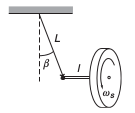
\includegraphics[width=2in]{img/8_3}
    \end{center}
\end{problem}
\begin{solution}
    \vfill
\end{solution}
\clearpage

\begin{problem}[Grain mill* - KK 8.4]
    In an old-fashioned rolling mill, grain is ground
    by a disk-shaped millstone that rolls in a circle 
    on a flat surface, driven by a vertical shaft. Because
    of the stone's angular momentum, the contact force 
    with the surface is greater than the weight of the wheel.

    Assume that the millstone is a uniform disk of mass $M$, 
    radius $b$, and width $w$, and that it rolls without 
    slipping in a circle of radius $R$ with angular speed 
    $\Omega$. Find the ratio of the contact force with respect
    to the surface to the weight of the stone.

    \begin{center}
        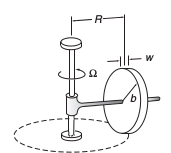
\includegraphics[width=2in]{img/8_4}
    \end{center}
\end{problem}
\begin{solution}
    \vfill
\end{solution}
\clearpage

\begin{problem}[Rolling coin* - KK 8.6]
    A coin of radius $b$ and mass $M$ rolls on a 
    horizontal surface at speed $V$. If the plane of
    the coin is vertical the coin rolls in a straight
    line. If the plane is tilted, the path of the coin
    is a circle of radius $R$. Find an expression for
    the tilt angle of the coin $\alpha$ in terms of
    the given quantities. (Because of the tilt of the
    coin the circle traced by its center of mass is 
    slightly smaller than $R$ but you can ignore the 
    difference.)

    \begin{center}
        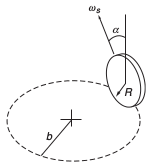
\includegraphics[width=2in]{img/8_6}
    \end{center}
\end{problem}
\begin{solution}
    \vfill
\end{solution}
\clearpage

\begin{problem}[Suspended hoop - KK 8.7]
    A thin hoop of mass $M$ and radius $R$ is suspended 
    from a string through a point on the rim of the hoop.
    If the support is turned with high angular velocity
    $\omega$, the hoop will spin as shown, with its plane 
    nearly horizontal and its center nearly on the axis of
    the support. The string makes angle $\alpha$ with the
    vertical.

    \begin{enumerate}[(a)]
        \item Find, approximately, the small angle $\beta$ between
            the plane of the hoop and the horizontal. Assume that
            the center of mass is at rest.
        \item Find, approximately, the radius of the small circle
            traced out by the center of mass about the vertical axis.
        \item Find a criterion for the validity of the assumption 
            that motion of the center of mass can be neglected. 
            (With skill you can demonstrate this with a rope. It is a
            favorite cowboy lariat trick.)
    \end{enumerate}

    \begin{center}
        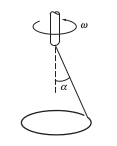
\includegraphics[width=1.5in]{img/8_7}
    \end{center}
\end{problem}
\begin{solution}
    \vfill
\end{solution}
\clearpage

\end{document}
